\section{Related Work}\label{sec:related_work}
% Your work needs to be grounded and compared to earlier work and the state-of-the-art. Start the section with announcing the research gap and also end with the research gap. Consider using hypotheses. 

\subsection{Gravitational Wave analysis}

The first direct detection of gravitational waves occurred in 2015 after the merger of two black holes about 1.3 billion light years away~\cite{LIGO_2016}. Since then, there have been three observing runs by the LIGO-Virgo collaboration which have yielded 90 confirmed gravitational wave detections . Of these 90 detections, 83 were binary black hole mergers, 2 were binary neutron star mergers, 3 were neutron star-black hole mergers and 2 involved the merger between a black hole and a `mystery' object that had a mass in between that of a neutron star and black hole~\cite{LIGO_FAQ_Website}. The next observing runs, O4 (started May 2023) and O5 (planned for 2027 and beyond) are predicted to detect a significant increase in events, $~\sim5\times$ more events each corresponding observing run~\cite{Petrov_2022}.

Analysis of gravitational waves is divided into two parts -- detection and parameter inference~\cite{bhardwaj2023peregrine}. In this study, we consider only the inference part, whereby given a detected waveform, we are trying to infer the physical properties of the source that generated it, as well as the distance, position and orientation in the sky relative to Earth etc.

\todo[inline]{Rewrite paragraph below}
The theory of how sources emit gravitational waves is well established, and the entire gravitational waveform may be expressed by $\sim$15 parameters~\cite{Thrane_Talbot_2019}. 
There are well established methods for accurately forward modelling GW waveforms, detector responses and instrument noise~\cite{alvey2023things} e.g.~the open-source Bilby code~\cite{Ashton_Bilby_2019,Romero_Bilby_2020,Ashton_Talbot_Bilby_2021}. Therefore, given the well-known theory, and these 15 parameters as input, it is fairly straightforward to accurately simulate what you expect the GW waveform to look like. However, performing the inverse of this problem i.e.~backing out the 15 parameters from a given GW waveform is significantly more challenging. Bayesian inference methods are therefore used extensively in gravitational-wave astronomy~\cite{Thrane_Talbot_2019}.

\todo[inline]{Rewrite paragraph below}
Due to the high dimensionality, brute-force techniques for GW parameter inference are computationally infeasible. The traditional approach involves using stochastic sampling methods~\cite{Thrane_Talbot_2019}, such as Markov chain Monte Carlo (MCMC)~\cite{Metropolis_1953,Hastings_1970} or nested sampling~\cite{Skilling_2004}. However, these techniques increasingly struggle with higher dimensional data and are not feasible options in the case of overlapping signals, where one needs to now infer 30 model parameters from the data~\cite{alvey2023things}.


\subsection{Swyft and Peregrine}



The \texttt{Peregrine} code was developed to study broad classes of gravitational wave signals. The papers describing the development of the code~\cite{bhardwaj2023peregrine,alvey2023things} will form the main starting point of this thesis, and will also serve as the baseline for this new work to be benchmarked against. \texttt{Peregrine} implements an SBI algorithm known as Truncated Marginal Neural Ratio Estimation (TMNRE)~\cite{Miller_TMNRE_2021} and is built on top of the \texttt{swyft} code~\cite{Miller2022}. The TMNRE algorithm estimates the marginal likelihood-to-evidence ratio, and works by training binary classifiers to distinguish jointly drawn sample pairs from marginally drawn sample pairs.

Summary statistics to MLP which calculates the log ratios.

\subsection{Neural Network Architectures}

\subsubsection{U-Net}

U-Net is a fully convolutional neural network that was originally developed in 2015 for biomedical image segmentation~\cite{Ronneberger_Fischer_Brox_2015}. U-Net is efficient and fast to train, and has thus become highly popular and the \enquote{gold standard} for segmenting 2D medical images for which new architectures should be benchmarked against~\cite{Sengara_2022}. The defining feature of U-Net is its symmetrical architecture consisting of a contracting path (encoder) followed by an expansive path (decoder). In the original U-Net~\cite{Ronneberger_Fischer_Brox_2015}, each step in the encoding path consists of two 3$\times$3 convolutions (unpadded in the original) doubling the number of feature channels, a ReLU and 2$\times$2 max pooling with stride 2 for downsampling. The decoding path then follows with a 2$\times$2 \enquote{up-convolution} halving the number of feature channels, concatenation with the matching feature map from the contractive path, followed by two 3$\times$3 convolutions and ReLU operations. The architecture of U-Net, reproduced from~\cite{Ronneberger_Fischer_Brox_2015}, is shown in Figure~\ref{fig:unet_arch}.

\begin{figure}
    \centering
    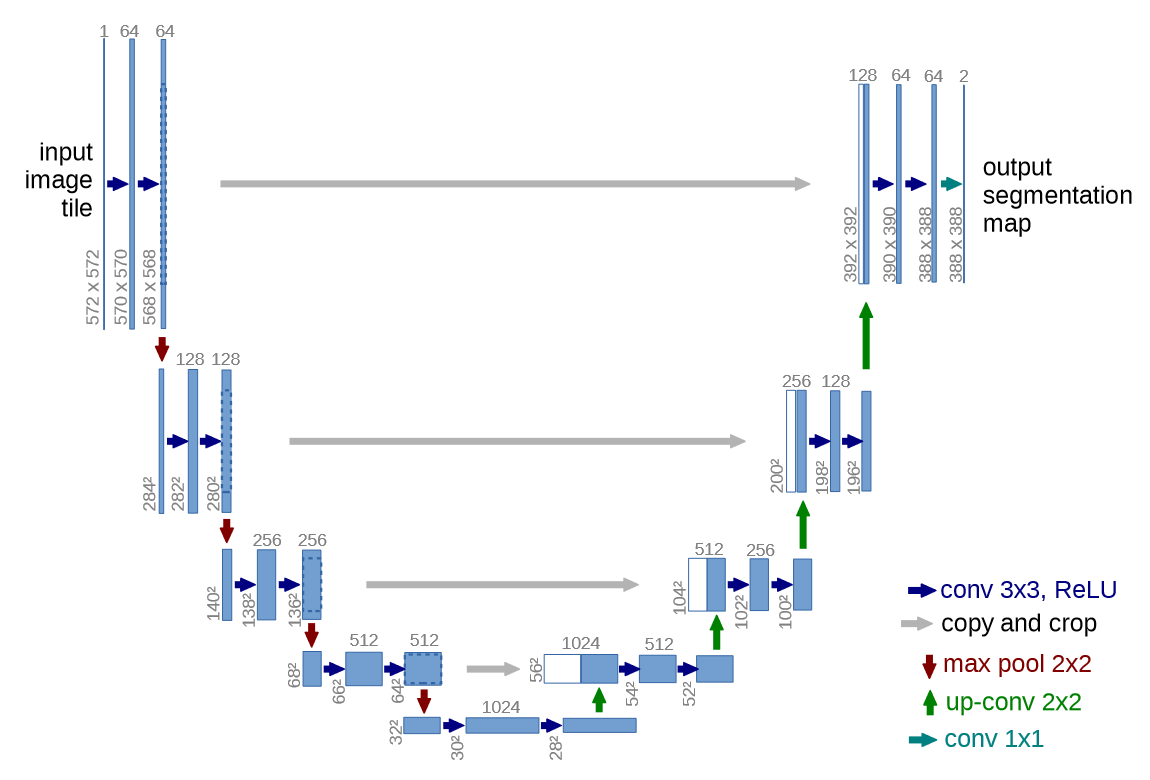
\includegraphics[width=1\linewidth]{media/images/UNet_arch.png}
    \caption{The U-Net architecture with a 2D image of resolution 572$\times$572 as example. Reproduced from~\cite{Ronneberger_Fischer_Brox_2015}.}
    \label{fig:unet_arch}
  \end{figure}

\subsubsection{Attention U-Net}

Due to the success of the U-Net architecture, several variants have since been proposed,including U-Net++~\cite{Zhou_2018_unet++} and attention U-Net~\cite{Oktay_2018_AUNet}. U-Net++
replaces the plane skip connections in vanilla U-Net with nested dense skip connections. This is to reduce the semantic gap between the encoder and decoder, which they claim yields significant performance gains.

The Attention U-Net introduces an attention gate (AG) in order to filter the features that are passed through the skip connections. The authors claim that this increases the models sensitivity and prediction accuracy with minimal impact to the computational cost. They do this by suppressing irrelevant features and learn to only focus on the most important features. 

Additive soft attention

\subsubsection{Transformer models}

Transformer models have proven widely succesful in the field of natural language progressing~\cite{Vaswani_2017_transformer} and computer vision~\cite{Dosovitskiy_2021_vit}. They provide a highly efficient platform for processing sequential data. Vision Transformers (ViT) have shown 

Vision transformers and time series models.

The use of transformer models for 1D signals is much less widespread, but~\cite{Nguyen_Miah_Bilodeau_Bouachir_2022} have shown they were very effective at extracting features from 1D signals, specifically detecting Parkinson's disease by analysing a patients gait. 

Transformers often require large amounts of training data and computing power before they are able to outperform task-specific models.

\subsection{Network pruning}

The implementation of attention U-Net and transformers models will increase the number of trainable parameters. This will likely place an additional overhead on the calculation time of \texttt{Peregrine} or require more training data. In order to reduce the number of model parameters pruning techniques exist such as \cite{Fang_Ma_Song_Mi_Wang_2023}.

